
\documentclass[UTF8,11pt,fontset=fandol]{ctexart}
\usepackage[a4paper,top=2.0cm,bottom=2.0cm,left=2.05cm,right=2.05cm]{geometry}
\usepackage{graphicx}
\usepackage{subcaption}
\usepackage{booktabs}
\usepackage{longtable}
\usepackage{tabularx}
\usepackage{array}
\usepackage{amsmath,amssymb}
\usepackage{siunitx}
\usepackage{xcolor}
\usepackage{hyperref}
\usepackage{enumitem}
\usepackage{caption}
\graphicspath{{./}}
\hypersetup{colorlinks=true,linkcolor=blue,citecolor=blue,urlcolor=blue}
\sisetup{detect-all=true,range-phrase=--,range-units=single}
\captionsetup{font=small,labelfont=bf}
\setlist{nosep,leftmargin=1.4em}
\renewcommand{\arraystretch}{1.18}
\title{二维聚合物薄膜的 AFM 力学测试、界面粘附与表观模量分析}
\author{}
\date{\today}

\begin{document}
\maketitle

\begin{abstract}
本报告基于二维聚合物薄膜的 AFM 力学测试数据，分别分析探针接近过程中的吸引力、回撤过程中的粘附与滞后行为，以及深压入加载曲线所反映的模型依赖表观膜力学性能。结果显示，JJS 样品在 approach/loading 段的吸引力中位数为 \SI{17.3}{nN}，四分位范围为 \SIrange{14.0}{20.7}{nN}，与半径 \SI{8}{nm} 探针下范德华力和毛细力的经典估算值 \SI{10.2}{nN} 同量级。相比之下，retract/unloading 段 pull-off 粘附力中位数达到 \SI{115.9}{nN}，约为 approach 吸引力的 \SI{7.0}{倍}，说明强信号主要来自接触后液桥/界面钉扎导致的回撤粘附和耗散。深压入结果进一步表明，不同表面活性剂或后处理会显著改变薄膜的有效承载网络：在同一 k80 系列内部，model-dependent apparent modulus 的排序为 PAA $>$ PFNA $>$ SDBS；linker2-PAA 在其测试条件下呈现更高且更稳定的 GPa 级表观膜模量。所有模量均解释为模型依赖的 apparent modulus，用于相对力学比较，而不直接等同于无缺陷材料的本征 Young's modulus。
\end{abstract}

\tableofcontents
\clearpage

\section{研究目标与数据概述}
\subsection{AFM 力曲线分析目标}
本文关注三个相互关联但物理来源不同的问题。第一，二维聚合物薄膜在 AFM 探针接近时产生多大的吸引力，以及该吸引力是否可由范德华力和毛细力的经典量级解释。第二，探针回撤时的 pull-off 粘附力和能量滞后有多强，它们反映的是接触后液桥拉伸、界面钉扎还是薄膜本身的弹性。第三，在排除 snap-in、pull-off 和明显不可恢复破裂后，深压入 loading 段能否给出表面活性剂依赖的相对薄膜力学性能。

\subsection{AFM 力曲线结构：approach/loading 与 retract/unloading}
每条 AFM 力曲线按加载和卸载分支分别处理。approach/loading 分支用于接近段吸引力、接触点和深压入力学；retract/unloading 分支用于 pull-off 粘附力、回撤面积和滞后功。这样的分支定义使吸附、粘附和弹性加载不再混在同一个物理量中。

\subsection{样品体系与表面处理组}
本报告包含 JJS、linker1、linker2 和 k80 系列样品。JJS 主要用于界面吸引力、粘附和滞后分析；linker2-PAA 和 k80 系列深压入曲线用于 apparent membrane mechanics。k80 系列内部的 PAA、PFNA 和 SDBS 对比是表面活性剂影响薄膜力学性能的主要证据。

\subsection{本报告可定量回答的科学问题}
可稳健定量的是 approach attraction scale、retract pull-off adhesion、pull-off/snap-in ratio、hysteresis work、stitched loading stiffness 和 model-dependent apparent modulus。effective capillary radius 与 Hamaker upper bound 只能作为半定量量级解释；真实水桥几何、单独 solvation force 和本征 Young's modulus 需要额外实验约束。

\begin{figure}[htbp]
    \centering
    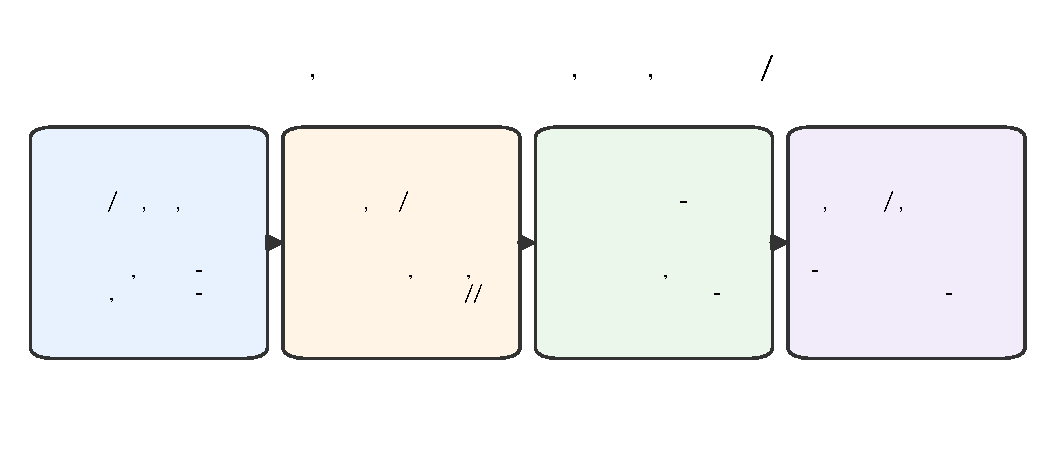
\includegraphics[width=0.96\linewidth]{workflow_scheme.pdf}
    \caption{AFM 力曲线分析流程图。加载分支用于接近段吸引力和深压入力学；卸载分支用于 pull-off 粘附和滞后功。}
    \label{fig:workflow}
\end{figure}

\begin{table}[htbp]
    \centering
    \caption{样品、探针参数与分析用途。}
    \label{tab:datasets}
    \small
    \begin{tabularx}{\linewidth}{lllclX}
        \toprule
        日期 & 主要样品 & 探针 & 半径 & 弹簧常数 & 主要用途 \\
        \midrule
        20260409 & JJS & RTESPA-150 & \SI{8}{nm} & \SI{7}{N/m} & approach 吸引力、retract 粘附、滞后与限域水桥候选机制 \\
        20260415 & linker1/linker2 & RTESPA-150 & \SI{8}{nm} & \SI{7}{N/m} & linker 系列粘附差异；linker2-PAA 深压入力学对照 \\
        20260416 & k80 系列 & DDESP-V2 & \SI{100}{nm} & \SI{89}{N/m} & PAA/PFNA/SDBS 表面活性剂 apparent mechanics 对比 \\
        \bottomrule
    \end{tabularx}
\end{table}

\section{力曲线处理方法}
\subsection{原始 Z-force 数据读取}
原始数据保留采集顺序，并记录源文件、分支、位移、setpoint、探针半径和弹簧常数。力统一转换为 nN，位移和压入深度统一为 nm；对于 uN 量级深压入曲线，先完成单位转换再进入同一套特征提取和拟合流程。

\subsection{extend 作为 approach/loading 曲线}
approach/loading 曲线用于 baseline 校正、snap-in/吸引力识别、接触点定位和 post-contact loading 分析。接近段吸引力以负力最小值的绝对值表示；深压入力学只取接触点之后的正力加载段。

\subsection{retract 作为 unloading/pull-off 曲线}
retract/unloading 曲线用于 pull-off 粘附力和回撤面积。pull-off force 定义为回撤分支中最强负力，其物理意义是接触形成之后的脱粘或液桥断裂强度，而不是接近段吸引力。

\subsection{baseline、contact、snap-in 与 pull-off 定义}
baseline 用远离表面的低相互作用区拟合并扣除。contact point 由基线后正力上升和局部斜率变化确定。snap-in 是 approach 分支中接触前后出现的负力极小值；pull-off 是 retract 分支中卸载阶段的负力极小值。work area 由相应曲线积分得到。

\subsection{有效曲线筛选与 QC 标准}
QC 标准包括 baseline 是否稳定、曲线点数是否足够、单位是否一致、深压入是否达到最小压入深度和正力阈值、膜模型拟合 $R^2$ 是否达标。含明显 baseline 风险或无足够 post-contact 点的曲线可用于定性查看，但不进入 apparent modulus 统计。

\section{Approach 吸引力：范德华力与毛细力}
\subsection{范德华吸引力模型}
探针靠近薄膜表面时，最基本的吸引力之一是球--平面范德华相互作用：
\begin{equation}
    F_\mathrm{vdW}=\frac{A R}{12 d_0^2},
    \label{eq:vdw}
\end{equation}
其中 $A$ 为有效 Hamaker 常数，$R$ 为探针半径，$d_0$ 为最小有效间距。该式适合做量级估算，不应在未知表面粗糙度和真实接触几何时过度反演 $A$。

\subsection{毛细桥力模型}
在空气湿度或亲水界面存在时，探针和薄膜之间可形成纳米水桥。完全润湿上限下，毛细力可写为
\begin{equation}
    F_\mathrm{cap}=4\pi R\gamma\cos\theta,
    \label{eq:capillary}
\end{equation}
其中 $\gamma$ 是水/空气界面张力，$\theta$ 为有效接触角。真实毛细力会受湿度、粗糙度、接触线钉扎和动态成核影响\cite{butt2005,israelachvili2011}。

\subsection{理论量级估算}
对 \SI{8}{nm} 半径探针，取 $A=4\times10^{-19}\ \mathrm{J}$、$d_0=\SI{0.3}{nm}$、$\gamma=\SI{72}{mN/m}$，得到 $F_\mathrm{vdW}\approx\SI{3.0}{nN}$、$F_\mathrm{cap}\approx\SI{7.2}{nN}$，二者合计约 \SI{10.2}{nN}。

\subsection{JJS extend 吸引力与理论模型对比}
JJS 样品 approach/loading 段吸引力中位数为 \SI{17.3}{nN}，四分位范围为 \SIrange{14.0}{20.7}{nN}。这个实测值只比经典 $F_\mathrm{vdW}+F_\mathrm{cap}$ 估算高约 1--2 倍，因此一个稍大的有效润湿半径、较强亲水界面、局部水桥成核或动态 snap-in 就足以解释观测量级。

\subsection{有效毛细半径与 Hamaker upper bound 的半定量解释}
如果把全部吸引力都写入 $F_\mathrm{cap}=4\pi R_\mathrm{eff}\gamma$，得到的是有效毛细半径，而不是真实几何半径。同样，如果把毛细力、静电和动态效应都并入式 \eqref{eq:vdw} 反推 $A$，得到的是 upper bound。二者只能用于判断物理量级，而不能作为唯一微观机制证明。

\begin{figure}[htbp]
    \centering
    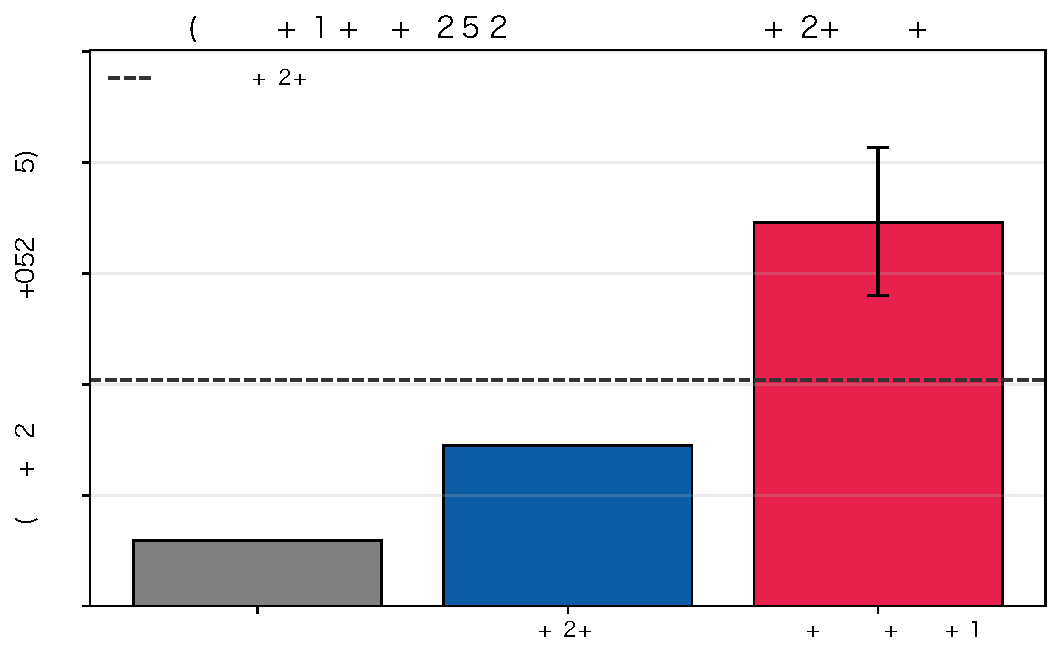
\includegraphics[width=0.82\linewidth]{approach_theory_comparison.pdf}
    \caption{JJS approach/loading 吸引力与 $F_\mathrm{vdW}+F_\mathrm{cap}$ 理论量级对比。}
    \label{fig:approach-theory}
\end{figure}

\section{Retract 粘附力与界面滞后}
\subsection{pull-off force 的定义}
pull-off force 是 unloading 曲线中最强负力，代表探针从已形成接触或液桥状态中脱离薄膜所需克服的最大粘附力。它反映的是接触后界面脱粘，而不是 approach 阶段的远程吸引力。

\subsection{JJS retract 粘附力统计}
JJS 的 retract/unloading pull-off 中位数为 \SI{115.9}{nN}，四分位范围为 \SIrange{108.2}{131.0}{nN}。该值远高于其 approach 吸引力，说明强信号主要发生在接触形成后的回撤阶段。

\subsection{extend attraction 与 retract adhesion 的不对称性}
JJS pull-off/snap-in 比值中位数为 \SI{7.0}{倍}。linker 系列和 k80 系列也表现出不同程度的加载/卸载不对称，说明薄膜界面不仅有可逆表面力，还有接触线钉扎、液桥拉伸、局部脱粘和耗散过程。

\subsection{滞后功计算}
对成对加载/卸载曲线，滞后功定义为
\begin{equation}
    W_\mathrm{hys}=\int_{\delta_1}^{\delta_2} F_\mathrm{load}(\delta)\,d\delta
    -
    \int_{\delta_1}^{\delta_2} F_\mathrm{unload}(\delta)\,d\delta .
    \label{eq:hysteresis}
\end{equation}
实际比较中使用 $|W_\mathrm{hys}|$ 表示耗散量级，避免符号约定影响结论。

\subsection{水桥拉伸、钉扎、延迟断裂与能量耗散机制}
最合理的物理图像是：接近时形成水桥或局部接触；回撤时水桥被拉伸，三相接触线在亲水/粗糙/缺陷位点上钉扎，导致负压、延迟断裂和明显能量耗散。当前数据支持限域水桥作为候选机制，但不能单独分离 solvation force、静电力和真实水桥几何。

\begin{figure}[htbp]
    \centering
    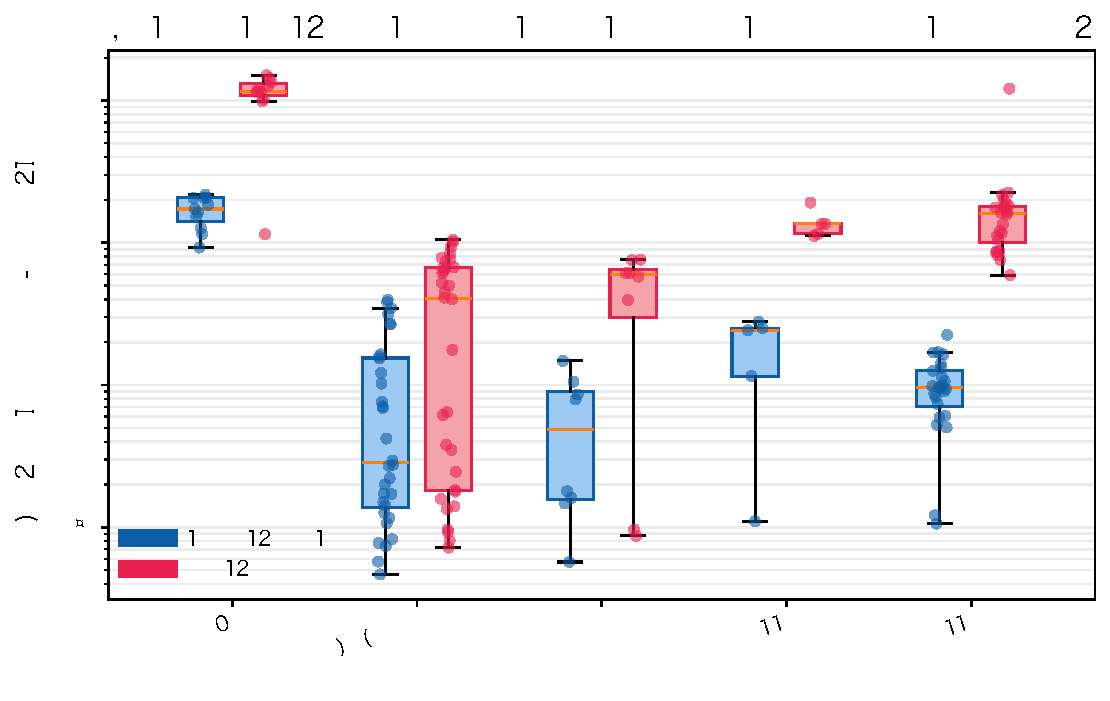
\includegraphics[width=0.95\linewidth]{branch_force_comparison.pdf}
    \caption{extend snap-in 与 retract pull-off 对比。纵轴为 log scale，用于同时展示 nN 到百 nN 量级差异。}
    \label{fig:branch-comparison}
\end{figure}

\begin{figure}[htbp]
    \centering
    
\includegraphics[width=0.86\linewidth]{hysteresis_ratio_work.pdf}
    \caption{pull-off/extend ratio 与 hysteresis work 分布。高比值和高耗散共同指向回撤阶段的液桥/界面钉扎贡献。}
    \label{fig:hysteresis}
\end{figure}

\section{样品间粘附差异}
\subsection{JJS 与 linker 系列粘附行为对比}
JJS 的回撤粘附显著强于其接近段吸引力，也强于多数 20260415 linker 系列。linker 系列中，PAA 相关样品通常具有更高 pull-off，提示亲水/带电界面对液桥稳定性和接触线钉扎具有增强作用。

\subsection{PAA、PFNA、SDBS 等表面处理的 pull-off ranking}
不同表面处理组的 pull-off ranking 反映了界面水桥、表面能和缺陷钉扎的共同作用。PAA 相关处理倾向于提高粘附；PFNA 和 SDBS 的粘附行为则与其表面化学、残留相和局部粗糙度有关。

\subsection{亲水性、粗糙度、缺陷与液桥稳定性的关系}
亲水性提高会降低水桥成核能垒；粗糙度和孔边缺陷会提供接触线钉扎位置；薄膜连续性和孔边界状态会影响回撤中水桥和局部接触能否稳定拉伸。因此，粘附差异不能只用单一参数解释，而应视为界面化学和形貌共同调控。

\subsection{粘附信号的可靠性与限制}
pull-off force 是本数据中较稳健的实验量，因为它来自回撤分支的清晰负力极值。限制在于它不是单一物理力：范德华、毛细、静电、局部塑性或脱粘都可能贡献。若要分离机制，需要湿度、干氮、不同探针半径和表面电势对照。

\begin{figure}[htbp]
    \centering
    
\includegraphics[width=0.82\linewidth]{adhesion_ranking.pdf}
    \caption{不同样品/处理组的 adhesion ranking。柱高为 retract pull-off 中位数。}
    \label{fig:adhesion-ranking}
\end{figure}

\begin{table}[htbp]
    \centering
    \caption{代表性样品的接近段吸引力和回撤段粘附力统计。数值为 median [Q1, Q3]。}
    \label{tab:adhesion}
    \small
    \begin{tabularx}{\linewidth}{lrrrr}
        \toprule
        组别 & 曲线对数 & approach 吸引力 / nN & retract 粘附力 / nN & pull-off/snap-in \\
        \midrule
        JJS & 11 & 17.29 [14.01, 20.68] & 115.92 [108.19, 130.95] & 7.02 [6.22, 7.60] \\
linker1-PFPE-OH & 32 & 0.28 [0.14, 1.55] & 4.06 [0.18, 6.72] & 3.13 [1.21, 5.37] \\
linker1-nls & 8 & 0.49 [0.16, 0.91] & 5.94 [2.99, 6.48] & 8.07 [3.26, 28.77] \\
linker1-paa & 5 & 2.43 [1.16, 2.51] & 13.57 [11.58, 13.59] & 7.87 [5.40, 9.66] \\
linker2-paa & 24 & 0.96 [0.70, 1.27] & 16.06 [10.05, 18.04] & 14.82 [12.01, 20.36] \\
        \bottomrule
    \end{tabularx}
\end{table}

\section{深压入曲线与滑脱拼接}
\subsection{深压入曲线筛选标准}
薄膜力学性能只从深压入正力 loading 段提取。候选曲线需要具有足够 post-contact 正力点、最大压入深度和最大排斥力达到深压入阈值，并且 baseline 与接触点识别没有明显失败。JJS 主要用于粘附/滞后分析，不作为 intrinsic mechanics 的主要来源。

\subsection{recoverable slip 与 terminal cliff 的分类}
recoverable slip 表现为力突然下降后，后续曲线重新回到上升趋势；terminal cliff 表现为末端大幅掉落且不恢复，通常对应破膜、脱粘或不可逆接触变化。前者可用于连续 loading 重构，后者只保留 cliff 前数据。

\subsection{垂直 force-offset stitching 方法}
对 recoverable slip 之后的整段曲线施加累计垂直 force offset，使 post-slip 段接到 pre-slip 趋势上。原始力值保留为 raw force；stitched force 只作为拟合视图。该方法不引入随机抖动，也不改变压入深度。

\subsection{拼接后 loading 曲线的力学用途}
stitched loading 曲线用于拟合 apparent stiffness、幂律指数和膜模型三次项。它的目标是尽可能恢复连续承载包络，从而避免可恢复滑脱导致的局部力下降把整体膜刚度低估。

\subsection{拼接方法的物理边界}
拼接不代表真实实验曲线被改写，也不能用于断裂强度分析。它只适合在 recoverable slip 明确、曲线仍保持整体 loading 趋势时使用；若出现不可恢复 cliff，则不对 cliff 之后做任何修复。

\begin{figure}[htbp]
    \centering
    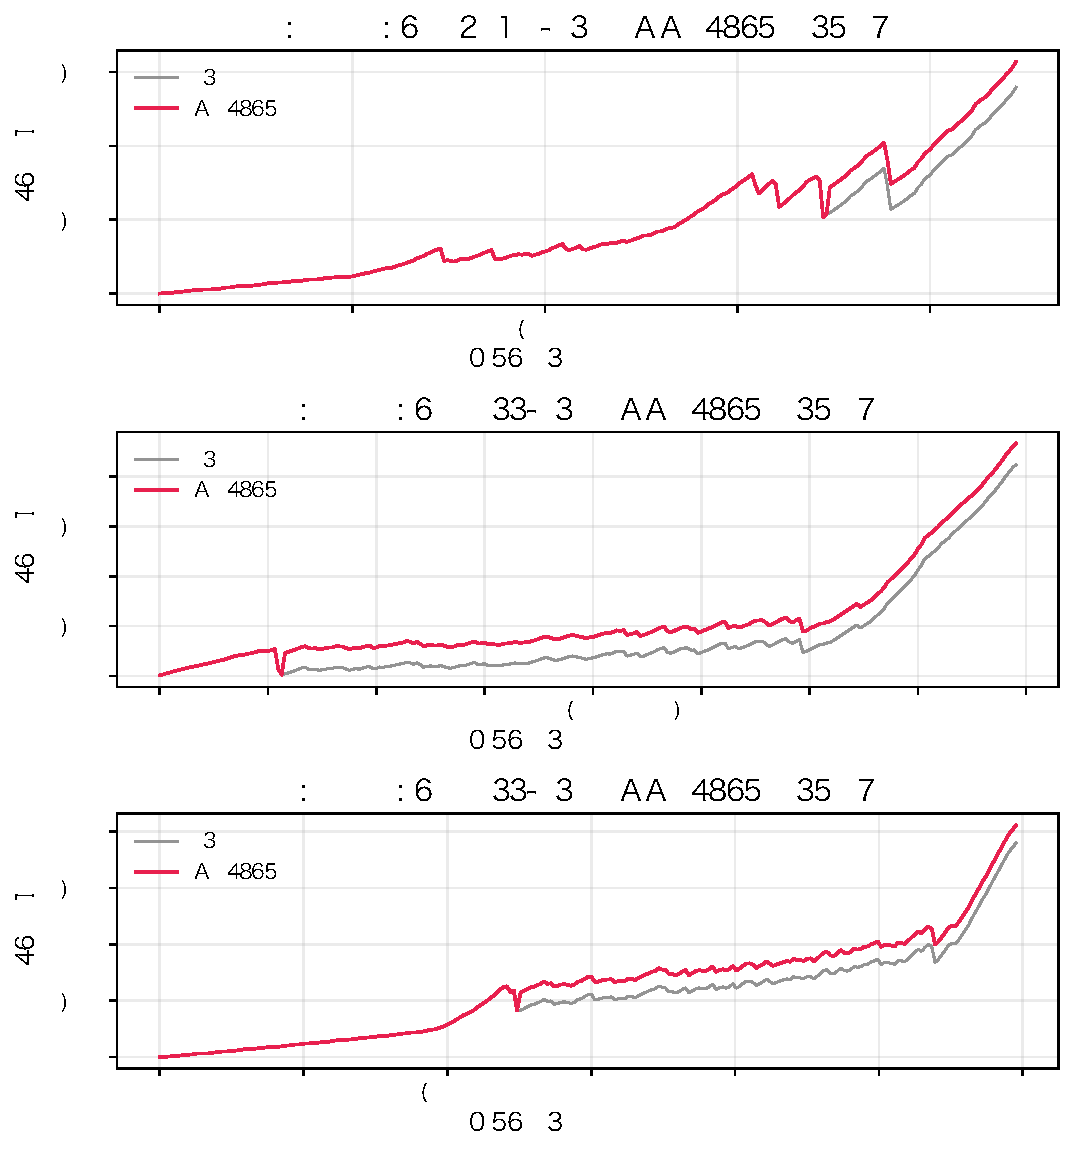
\includegraphics[width=0.92\linewidth]{stitch_raw_vs_stitched_examples.pdf}
    \caption{深压入曲线拼接前后对比。灰色为原始 loading 点，红色为 stitched loading 视图。}
    \label{fig:stitch}
\end{figure}

\begin{figure}[htbp]
    \centering
    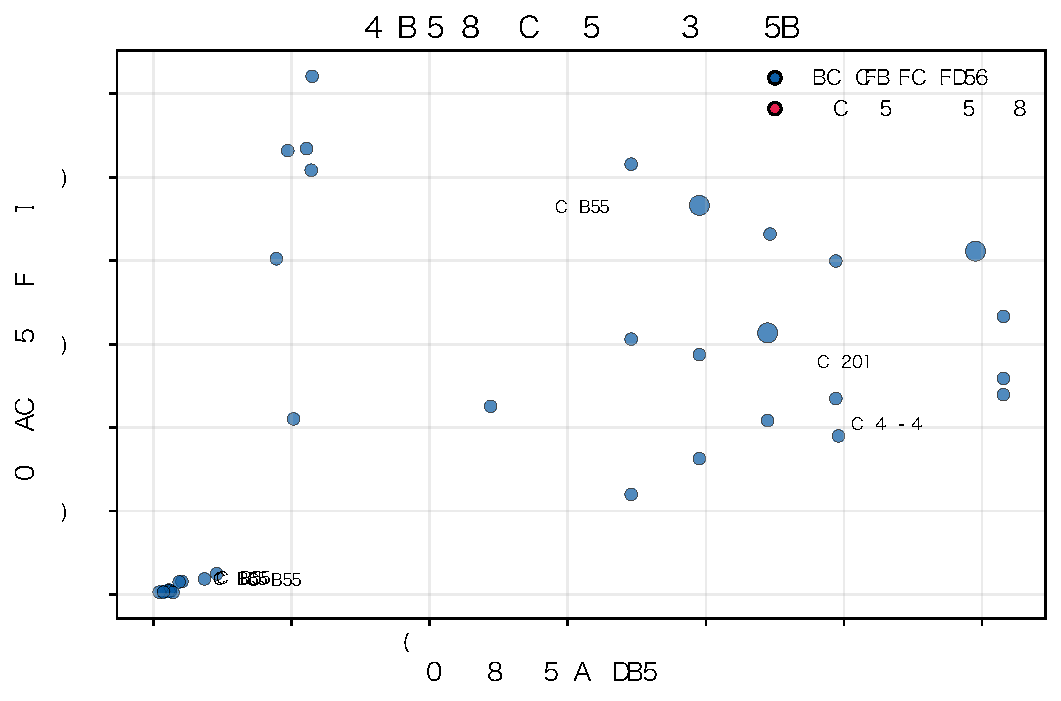
\includegraphics[width=0.82\linewidth]{slip_event_map.pdf}
    \caption{滑脱事件分布图。点大小随 recoverable slip 数量增加；红色表示 terminal cliff 标记。}
    \label{fig:slip-map}
\end{figure}

\section{薄膜力学模型}
\subsection{apparent low-force stiffness 与 high-force stiffness}
深压入段首先给出经验刚度：
\begin{equation}
    k_\mathrm{low}=\left.\frac{dF}{d\delta}\right|_\mathrm{low\ force},
    \qquad
    k_\mathrm{high}=\left.\frac{dF}{d\delta}\right|_\mathrm{high\ force} .
    \label{eq:stiffness}
\end{equation}
$k_\mathrm{low}$ 对接触点、预张力和局部顺应性敏感；$k_\mathrm{high}$ 更接近大压入下的承载能力。二者比值描述 strain-stiffening 或 loading 非线性。

\subsection{幂律模型}
幂律模型写为
\begin{equation}
    F=A\delta^n .
    \label{eq:powerlaw}
\end{equation}
指数 $n$ 可作为经验指标：$n$ 接近 1 表示近似线性刚度；较高 $n$ 表示大变形膜拉伸、几何非线性或接触面积变化增强。

\subsection{clamped circular membrane 模型}
主报告采用夹持圆形悬膜的 AFM 压入模型\cite{lee2008,bertolazzi2011}：
\begin{equation}
    F=k_1\delta+k_3\delta^3 .
    \label{eq:membrane-fit}
\end{equation}
线性项 $k_1\delta$ 合并了预张力、边界顺应性和低压入接触刚度；三次项 $k_3\delta^3$ 反映大变形膜拉伸主导的非线性承载。

\subsection{model-dependent apparent Young's modulus}
若把二维拉伸模量写为 $E_{2D}=E t$，夹持圆膜近似给出
\begin{equation}
    k_3=\frac{E_\mathrm{app} t q^3}{a^2},
    \qquad
    q=\frac{1}{1.05-0.15\nu-0.16\nu^2},
    \label{eq:k3}
\end{equation}
因此
\begin{equation}
    E_\mathrm{app}=\frac{k_3a^2}{q^3t} .
    \label{eq:eapp}
\end{equation}
单位换算中，若 $k_3$ 由 nN/nm$^3$ 拟合得到，则 $k_3[\mathrm{N/m^3}]=10^{18}k_3[\mathrm{nN/nm^3}]$。

\subsection{膜厚、孔径和泊松比的参数敏感性}
本文默认孔半径 $a=\SI{10}{\micro\meter}$、泊松比 $\nu=0.30$、主膜厚 $t=\SI{50}{nm}$，并给出 $t=\SI{80}{nm}$ 的敏感性估计。由于 $E_\mathrm{app}\propto a^2/t$，孔径误差会平方放大，膜厚误差会线性传递。

\subsection{为什么结果应解释为 apparent modulus}
$E_\mathrm{app}$ 不是严格本征 Young's modulus，因为 AFM 探针几何、薄膜缺陷、厚度不均、边界夹持顺应性和可恢复滑脱都会进入拟合参数。它最适合用于同一探针、同一批次、同一模型下的相对力学排序。

\begin{figure}[htbp]
    \centering
    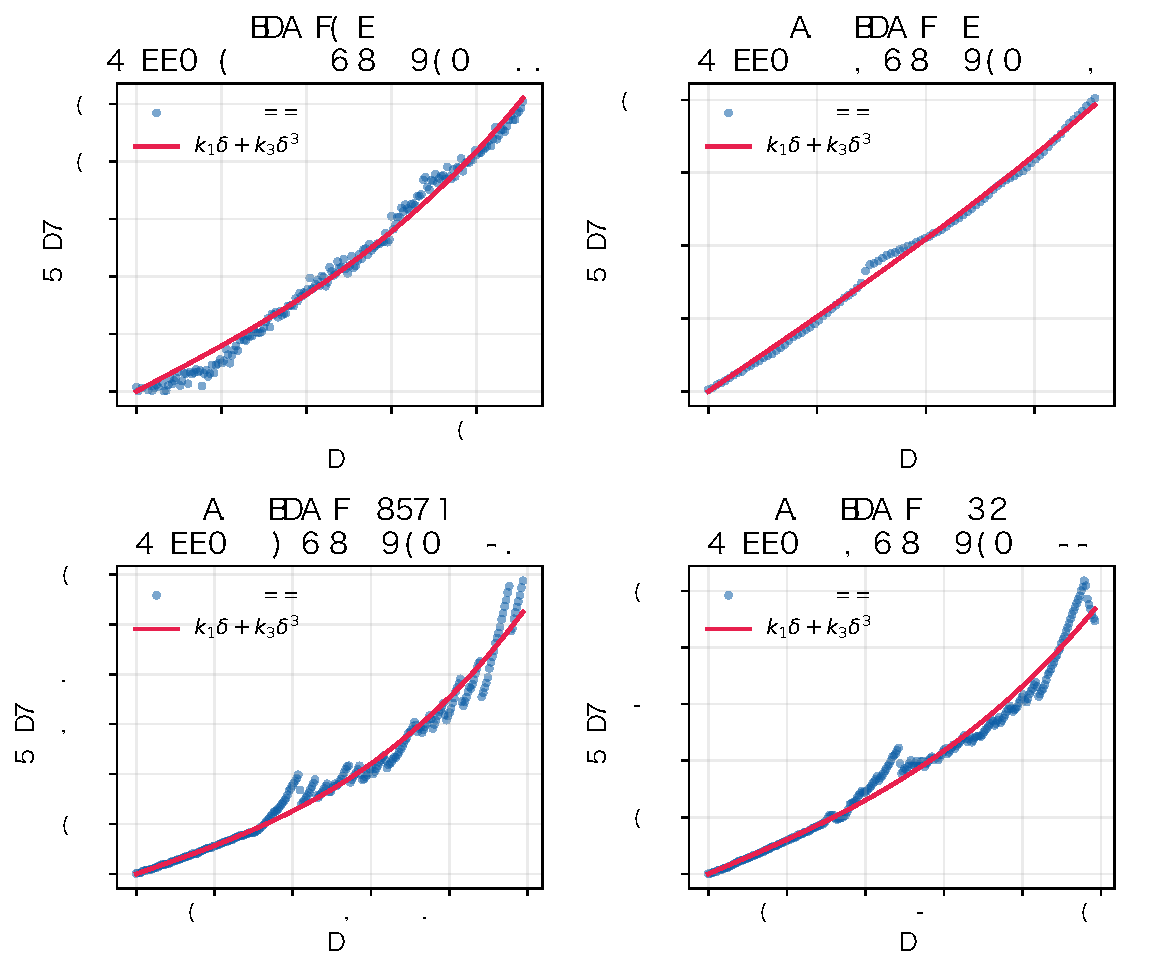
\includegraphics[width=0.96\linewidth]{membrane_model_fit_examples.pdf}
    \caption{代表性膜模型拟合曲线。}
    \label{fig:fits}
\end{figure}

\begin{figure}[htbp]
    \centering
    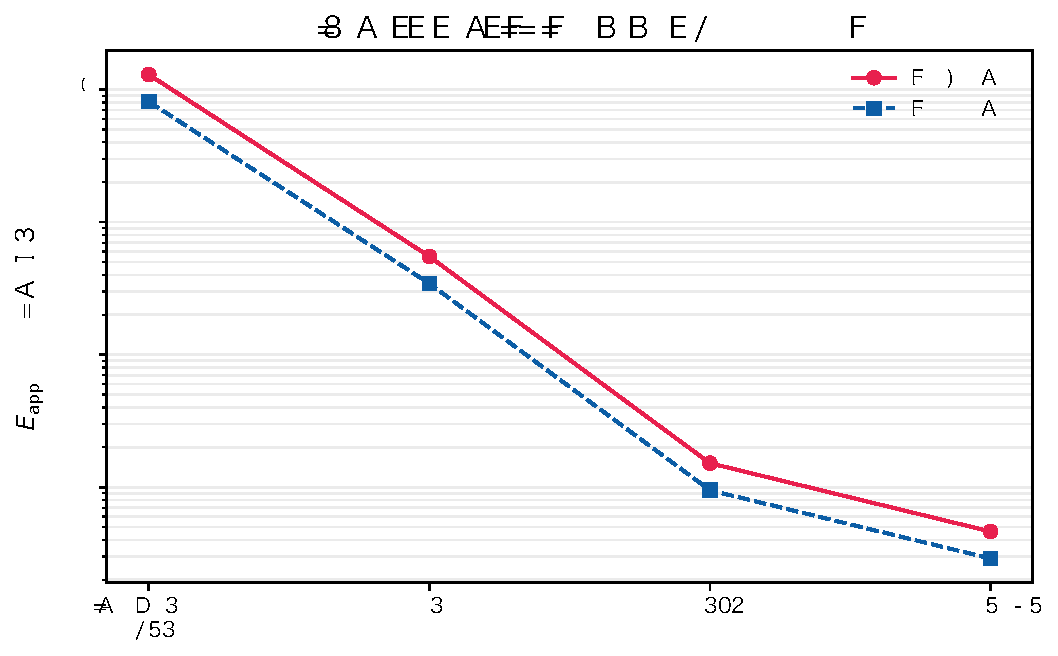
\includegraphics[width=0.82\linewidth]{thickness_sensitivity.pdf}
    \caption{膜厚敏感性分析。由于 $E_\mathrm{app}\propto 1/t$，80 nm 假设下的模量低于 50 nm 主值。}
    \label{fig:thickness}
\end{figure}

\section{表面活性剂对薄膜力学性能的影响}
\subsection{k80-linker1-paa 力学表现}
在同一 k80 系列内部，PAA 处理组的 apparent modulus 和高力区刚度最高。PAA 组中位 $E_\mathrm{app}$ 为几十 MPa，且部分曲线达到更高承载力，说明其悬膜在大压入下更能维持连续拉伸网络。

\subsection{k80-linker1-PFNA 力学表现}
PFNA 组的 $E_\mathrm{app}$ 比 PAA 明显降低，处于低 MPa 量级。该结果提示 PFNA 处理可能产生较弱的有效承载路径、更多局部软化区域或较低界面结合。

\subsection{k80-linker1-SDBS 力学表现}
SDBS 组有效曲线数较少，但现有有效曲线显示亚 MPa 到低 MPa 的 apparent modulus，整体低于 PAA 和 PFNA。该组应标注 low-N 风险，并避免过度解释绝对值。

\subsection{linker2-paa 的有效曲线数量与可靠性}
linker2-PAA 在其测试条件下表现出更高且更稳定的 GPa 级 apparent modulus，有效曲线数为 15，膜模型 $R^2$ 中位数接近 0.99。这提示 linker2-PAA 形成的悬膜网络更连续，深压入加载时可进入稳定拉伸主导区。

\subsection{apparent modulus ranking}
跨日期、跨探针结果只作量级参考；同一 k80 系列内部的排序最可靠：PAA $>$ PFNA $>$ SDBS。linker2-PAA 显示高可重复性，但因探针半径和测试条件不同，不宜直接与 k80 系列做绝对优劣判断。

\subsection{表面形貌、缺陷密度与膜连续性的结构-性能关系}
表面活性剂可能通过改变晶粒融合、片层堆积、残留相分离、孔洞和界面脱粘位置来改变薄膜力学表现。PAA 更高的刚度和模量提示更连续的承载网络；PFNA/SDBS 的低模量则更符合缺陷密度更高或有效承载路径更少的情形。该因果链仍需形貌和膜厚证据闭合。

\begin{figure}[htbp]
    \centering
    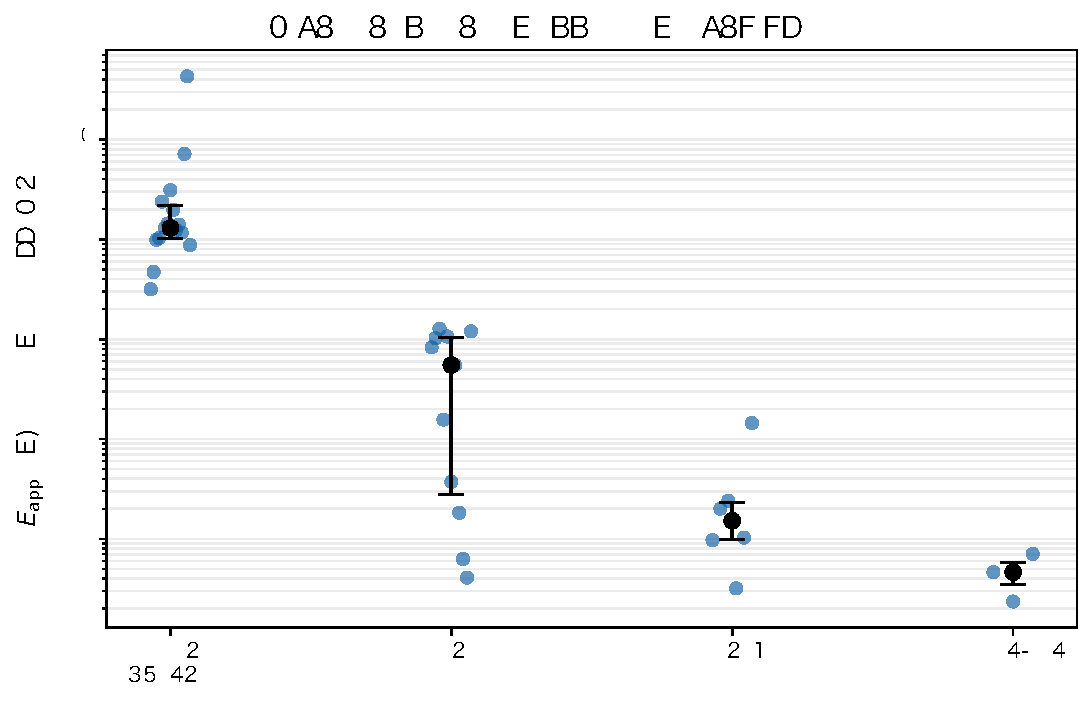
\includegraphics[width=0.88\linewidth]{apparent_modulus_ranking.pdf}
    \caption{不同表面活性剂 $E_\mathrm{app}$ boxplot/散点图。黑点和误差棒表示中位数与 IQR。}
    \label{fig:modulus-ranking}
\end{figure}

\begin{figure}[htbp]
    \centering
    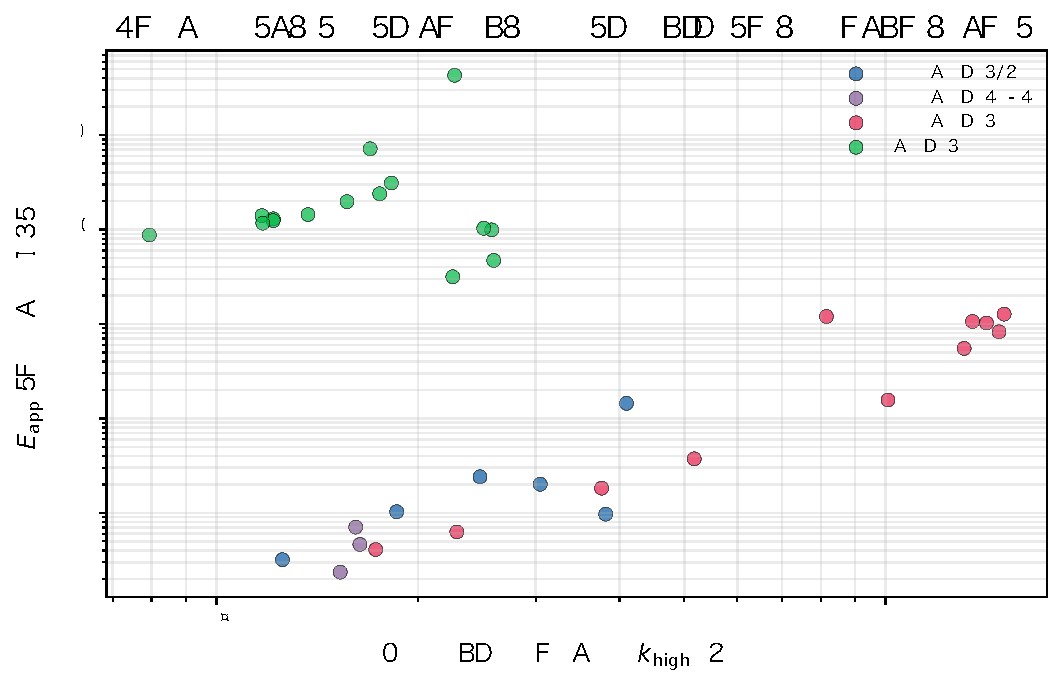
\includegraphics[width=0.82\linewidth]{stiffness_vs_modulus.pdf}
    \caption{apparent stiffness vs apparent modulus。高力区刚度和三次项模量相关，但二者受不同模型假设影响。}
    \label{fig:stiffness-vs-modulus}
\end{figure}

\begin{table}[htbp]
    \centering
    \caption{各处理组 $E_\mathrm{app}$、有效曲线数与 QC。$E_\mathrm{app}$ 为 median [Q1, Q3]，主值取 $t=\SI{50}{nm}$。}
    \label{tab:mechanics}
    \small
    \setlength{\tabcolsep}{3.5pt}
    \begin{tabularx}{\linewidth}{llrrrrr}
        \toprule
        日期 & 组别 & 有效曲线 & $E_\mathrm{app}$ 50 nm / MPa & $E_\mathrm{app}$ 80 nm / MPa & $k_\mathrm{high}$ / N m$^{-1}$ & $R^2$ \\
        \midrule
        20260415 & linker2-PAA & 15 & 1299.139 [1011.447, 2184.340] & 811.962 & 0.170 & 0.988 \\
20260416 & k80-linker1-PAA & 11 & 55.064 [2.778, 104.348] & 34.415 & 1.007 & 0.994 \\
20260416 & k80-linker1-PFNA & 6 & 1.517 [0.982, 2.308] & 0.948 & 0.276 & 0.972 \\
20260416 & k80-linker1-SDBS & 3 & 0.463 [0.349, 0.584] & 0.289 & 0.161 & 0.976 \\
20260416 & k80-linker2-PAA & 0 & -- [--, --] & -- & -- & -- \\
        \bottomrule
    \end{tabularx}
\end{table}

\section{误差棒与统计表达}
\subsection{曲线间变异：median 与 IQR}
本报告以每条有效曲线为统计单元，中心值使用 median，误差棒使用 interquartile range。该表达直接反映样品内部不均一性和缺陷导致的曲线间变异。

\subsection{模型拟合误差：$R^2$、残差与 confidence interval}
膜模型拟合质量用 $R^2$ 和残差趋势评估。$R^2$ 高说明 $k_1\delta+k_3\delta^3$ 能描述 stitched loading 包络，但不代表模型假设完全真实。后续可用 bootstrap 或曲线内残差重采样给出 $k_3$ confidence interval。

\subsection{膜厚不确定性：50--80 nm 敏感性范围}
由于 $E_\mathrm{app}\propto 1/t$，膜厚从 50 nm 增至 80 nm 会使 apparent modulus 乘以 $50/80=0.625$。因此图表同时给出 50 nm 主值和 80 nm 敏感性值。

\subsection{low-N 数据的标注方式}
有效曲线数 $N<5$ 的组只做趋势性讨论，不作为强统计结论。SDBS 和 k80-linker2-PAA 等低 N 或无有效模型组需要在图注和表格中明确标注。

\subsection{推荐图示：单曲线散点 + median + IQR}
推荐所有组间力学图采用单曲线散点叠加 median+IQR，而不是只画均值柱状图。这样能同时展示中心趋势、离散度和异常高/低曲线。

\begin{figure}[htbp]
    \centering
    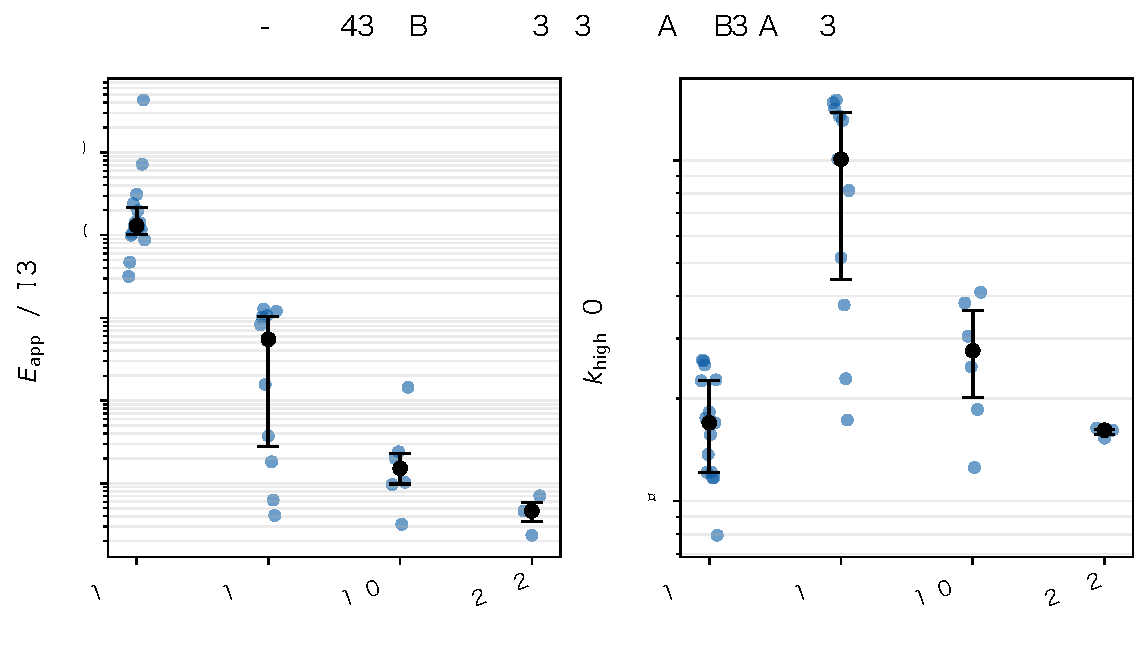
\includegraphics[width=0.90\linewidth]{median_iqr_errorbars.pdf}
    \caption{带原始散点、median 和 IQR 的力学性能图。}
    \label{fig:errorbars}
\end{figure}

\section{与其他薄膜材料的量级比较}
\subsection{软聚合物薄膜}
PDMS 类软弹性体常见 Young's modulus 约为 \SIrange{1}{3}{MPa}\cite{pdms2023}。k80-PFNA 和 k80-SDBS 接近这一软材料区间，而 k80-PAA 明显更硬。

\subsection{水凝胶/软界面薄膜}
水凝胶通常处于 kPa 到低 MPa 区间\cite{hydrogel2024,su2016}。本体系中较软的表面活性剂组接近软凝胶/弹性体边界，说明缺陷和界面弱连接可显著降低悬膜承载能力。

\subsection{超薄无机/有机复合膜}
linker2-PAA 的 GPa 量级 apparent modulus 接近刚性聚合物薄膜或部分多孔有机薄膜，但仍低于高度取向、缺陷极少的二维晶体材料。

\subsection{本体系 apparent modulus 的合理性与特殊性}
当前薄膜的力学量级位于软凝胶/弹性体与高模量二维晶体之间，这与其多孔、多晶、界面处理和可能存在缺陷的结构相符。核心发现不是达到无缺陷二维晶体极限，而是表面化学使实际承载路径跨越多个数量级。

\subsection{对表面活性剂调控缺陷和力学性能的启示}
表面活性剂可以通过成膜形貌、缺陷密度、界面润湿和边界结合改变 apparent modulus。这为文章主线提供了结构--性能关系：表面活性剂改变形貌和缺陷，缺陷改变有效承载网络，最终改变 AFM 深压入力学响应。

\begin{figure}[htbp]
    \centering
    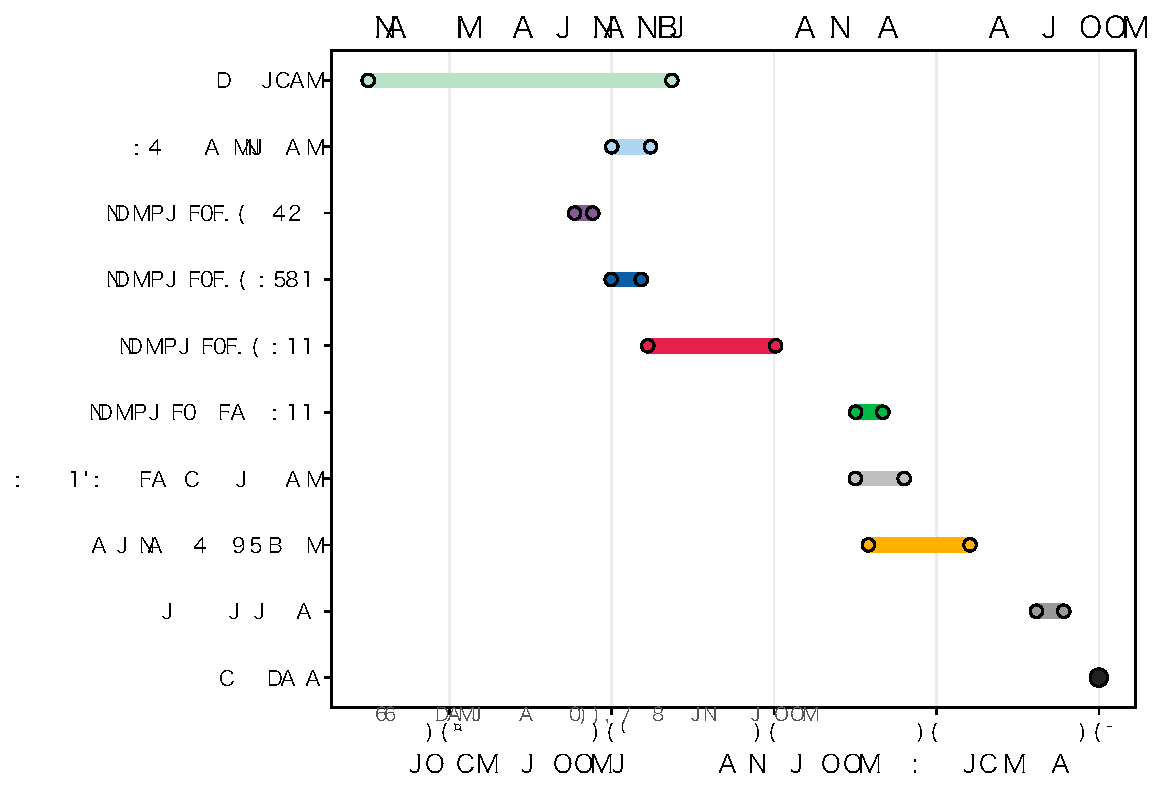
\includegraphics[width=0.92\linewidth]{literature_modulus_context.pdf}
    \caption{本体系 apparent modulus 与文献中典型薄膜材料模量范围对比。文献值仅作尺度参照。}
    \label{fig:literature}
\end{figure}

\section{可提取物理量与科学结论}
\subsection{可稳健提取的量}
可稳健提取 approach attraction scale、retract pull-off adhesion、hysteresis work、apparent membrane stiffness 和 model-dependent apparent modulus ranking。这些量直接来自分支清晰的力曲线特征或深压入拟合。

\subsection{半定量物理量}
effective capillary contribution、effective Hamaker upper bound 和 apparent tension/stress 可作为半定量指标。它们对模型假设敏感，不能单独作为微观机制证明。

\subsection{当前不宜单独定量的量}
单独 solvation force、真实水桥几何、破膜强度和本征 Young's modulus 目前不可可靠提取。前两者需要环境和表面电势对照；破膜强度需要明确 terminal cliff 的物理来源；本征模量需要独立膜厚、孔径、边界和接触模型约束。

\begin{table}[htbp]
    \centering
    \caption{可提取、半定量与不可可靠提取物理量总结。}
    \label{tab:extractability}
    \small
    \begin{tabularx}{\linewidth}{lll}
        \toprule
        类别 & 物理量 & 解释边界 \\
        \midrule
        可稳健提取 & approach attraction scale & 远程吸引力加动态 snap-in 的量级 \\
        可稳健提取 & retract pull-off adhesion & 接触后脱粘/液桥断裂强度 \\
        可稳健提取 & hysteresis work & 加载/卸载耗散量级 \\
        可稳健提取 & apparent modulus ranking & 同模型下相对薄膜承载能力 \\
        半定量 & effective capillary radius & 吸收润湿、粗糙和水桥几何的有效参数 \\
        半定量 & effective Hamaker upper bound & 会混入毛细和静电贡献 \\
        不可靠单独提取 & solvation force / true bridge geometry & 需要湿度、干氮、KPFM 或探针半径系列 \\
        不可靠单独提取 & intrinsic Young's modulus & 需要独立膜厚、边界和接触模型验证 \\
        \bottomrule
    \end{tabularx}
\end{table}

\section{总结与文章主线}
\subsection{AFM 力学测试揭示的二维聚合物薄膜界面粘附行为}
接近段吸引力处于范德华力加毛细力的合理量级；真正显著的界面非对称性出现在回撤粘附和滞后中。JJS 的强 pull-off 支持液桥拉伸、界面钉扎和延迟断裂的物理图像。

\subsection{表面活性剂改变薄膜缺陷与形貌，从而改变 apparent mechanics}
深压入结果说明表面活性剂和后处理会显著改变悬膜有效承载网络。PAA 相关样品通常表现出更强承载能力；PFNA 和 SDBS 则显示更软的 apparent mechanics。

\subsection{深压入数据支持的相对力学排序}
同一 k80 系列内部最可靠的排序为 PAA $>$ PFNA $>$ SDBS。linker2-PAA 在自身测试条件下显示最高可重复性和 GPa 级 apparent modulus，但不与 k80 系列做绝对优劣比较。

\subsection{后续实验建议：膜厚、形貌、湿度、探针半径与重复性验证}
后续应补充膜厚统计、AFM height/phase 或 SEM/TEM 形貌、湿度/干氮对照、不同探针半径测试和更大样本量。这样可以把 AFM 力曲线中的相对力学排序与“表面活性剂--形貌/缺陷--薄膜力学性能”的因果链更牢固地连接起来。

\appendix
\section{公式推导}
从夹持圆膜大变形压入模型出发，力可分解为线性项和几何非线性项 $F=k_1\delta+k_3\delta^3$。若二维模量 $E_{2D}=Et$，圆膜半径为 $a$，泊松比修正因子为 $q$，则三次项满足 $k_3=E_\mathrm{app}tq^3/a^2$，整理得到 $E_\mathrm{app}=k_3a^2/(q^3t)$。该公式是本报告 apparent modulus 的唯一换算公式。

\section{曲线处理与拼接算法}
拼接算法只检测 post-contact 正力 loading 段中的可恢复负向突跳。对每个 recoverable slip，计算跳落前趋势和跳落后恢复段之间的力差，并对后续整段施加累计垂直 offset。terminal cliff 后数据被截断，不参与拟合。

\section{曲线级 QC 与完整统计表}
曲线级统计保存在结果表中，包括 baseline 状态、最大压入、最大排斥力、slip 事件数、terminal cliff 标记、拟合点数、$k_1$、$k_3$、$R^2$、$E_\mathrm{app}$ 和 QC warning。正文只报告通过模型 QC 的曲线统计。

\section{图表生成参数}
所有图为 A4 报告重新生成，单栏图宽约为正文宽度的 0.82--0.96 倍，字体约 10--14 pt。力单位为 nN，长度单位为 nm，apparent modulus 主值使用 $a=\SI{10}{\micro\meter}$、$t=\SI{50}{nm}$、$\nu=0.30$，并给出 $t=\SI{80}{nm}$ 敏感性。

\begin{thebibliography}{9}
\bibitem{butt2005}
Butt, H.-J.; Cappella, B.; Kappl, M. Force measurements with the atomic force microscope: Technique, interpretation and applications. \textit{Surface Science Reports} \textbf{2005}, 59, 1--152. \url{https://doi.org/10.1016/j.surfrep.2005.08.003}

\bibitem{israelachvili2011}
Israelachvili, J. N. \textit{Intermolecular and Surface Forces}, 3rd ed.; Academic Press, 2011. \url{https://doi.org/10.1016/C2011-0-05119-0}

\bibitem{lee2008}
Lee, C.; Wei, X.; Kysar, J. W.; Hone, J. Measurement of the elastic properties and intrinsic strength of monolayer graphene. \textit{Science} \textbf{2008}, 321, 385--388. \url{https://doi.org/10.1126/science.1157996}

\bibitem{bertolazzi2011}
Bertolazzi, S.; Brivio, J.; Kis, A. Stretching and breaking of ultrathin MoS$_2$. \textit{ACS Nano} \textbf{2011}, 5, 9703--9709. \url{https://doi.org/10.1021/nn203879f}

\bibitem{hydrogel2024}
Jagiełło, J.; et al. A comprehensive mechanical testing of polyacrylamide hydrogels: The impact of crosslink density. \textit{Gels} \textbf{2024}. \url{https://pmc.ncbi.nlm.nih.gov/articles/PMC11944691/}

\bibitem{su2016}
Su, T.; Liu, Y.; He, H.; Li, J.; Lv, Y.; Zhang, L.; Sun, Y.; Hu, C. Strong bioinspired polymer hydrogel with tunable stiffness and toughness for mimicking the extracellular matrix. \textit{ACS Macro Letters} \textbf{2016}, 5, 1217--1221. \url{https://doi.org/10.1021/acsmacrolett.6b00702}

\bibitem{pdms2023}
Liu, M.; et al. Functional PDMS elastomers: Bulk composites, surface engineering, and precision fabrication. \textit{Advanced Science} \textbf{2023}. \url{https://pmc.ncbi.nlm.nih.gov/articles/PMC10700310/}

\bibitem{cof2025}
Xiong, L.; Fu, C.; Tian, J.; Geng, Y.; Han, L.; Zhang, H.; Li, H. Intrinsic mechanical properties of two-dimensional covalent organic frameworks. \textit{Chemical Science} \textbf{2025}, 16, 15913--15925. \url{https://doi.org/10.1039/D5SC02180D}
\end{thebibliography}

\end{document}
